
\section{modelling}

\subsection{overview}



\begin{figure}[h]
 \centering
 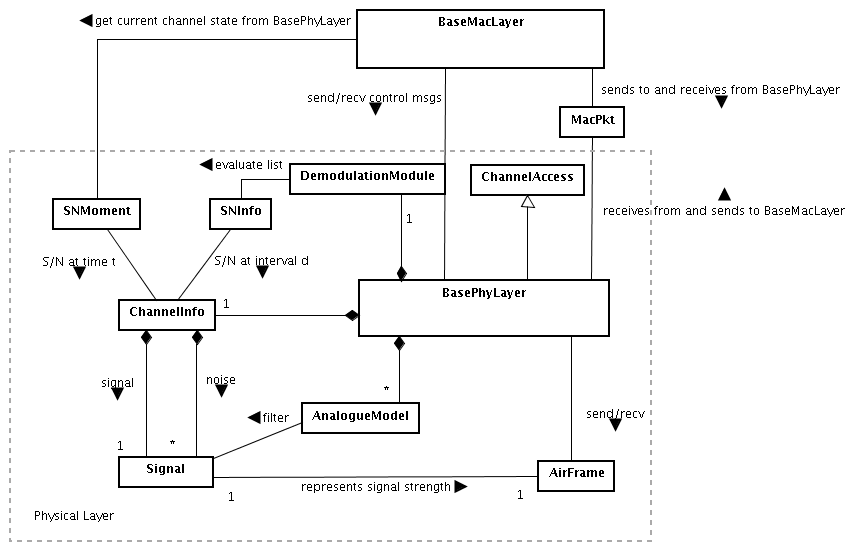
\includegraphics[width=400pt]{modelling/class_diagram.png}
 \caption{class graph}
 \label{fig: class graph}
\end{figure}

\begin{figure}[h]
 \centering
 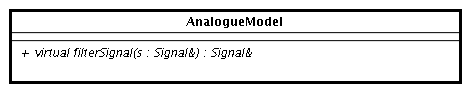
\includegraphics[width=340pt]{modelling/AnalogueModel_members.png}
 \caption{analogue model interface}
 \label{fig: analogue model interface}
\end{figure}

\begin{figure}[h]
 \centering
 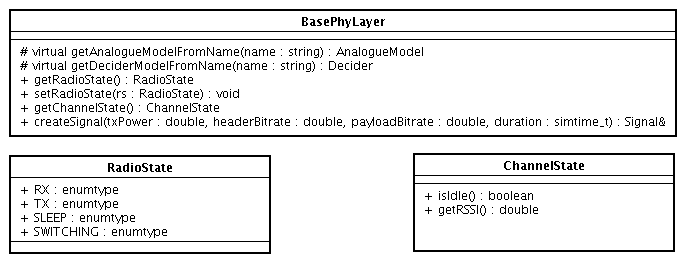
\includegraphics[width=340pt]{modelling/BasePhyLayer_members.png}
 \caption{BasePhyLayer interface}
 \label{fig: BasePhyLayer interface}
\end{figure}

\begin{figure}[h]
 \centering
 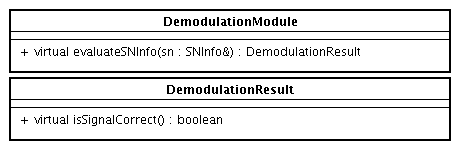
\includegraphics[width=340pt]{modelling/DemodulationModule_members.png}
 \caption{Demodulator interface}
 \label{fig: Demodulator interface}
\end{figure}

\begin{figure}[h]
 \centering
 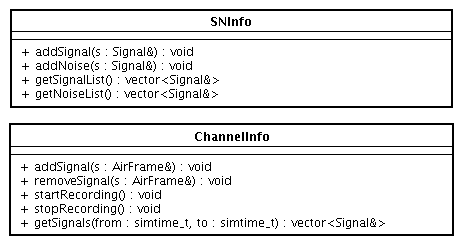
\includegraphics[width=340pt]{modelling/ChannelInfo_members.png}
 \caption{channel details}
 \label{fig: channel details}
\end{figure}

\begin{figure}[h]
 \centering
 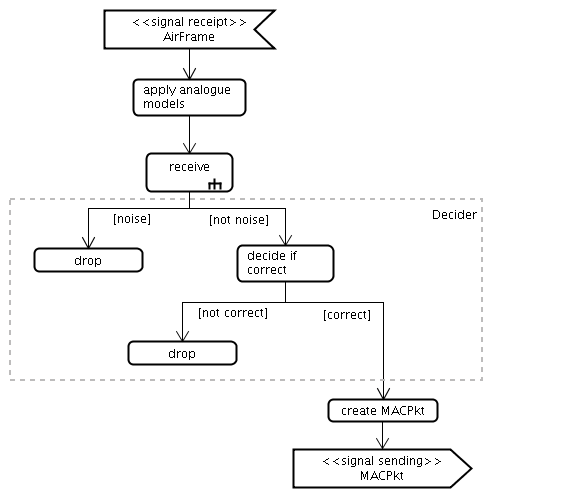
\includegraphics[width=340pt]{modelling/onAirFrame.png}
 \caption{receiving process}
 \label{fig: receiving process}
\end{figure}

\begin{figure}[h]
 \centering
 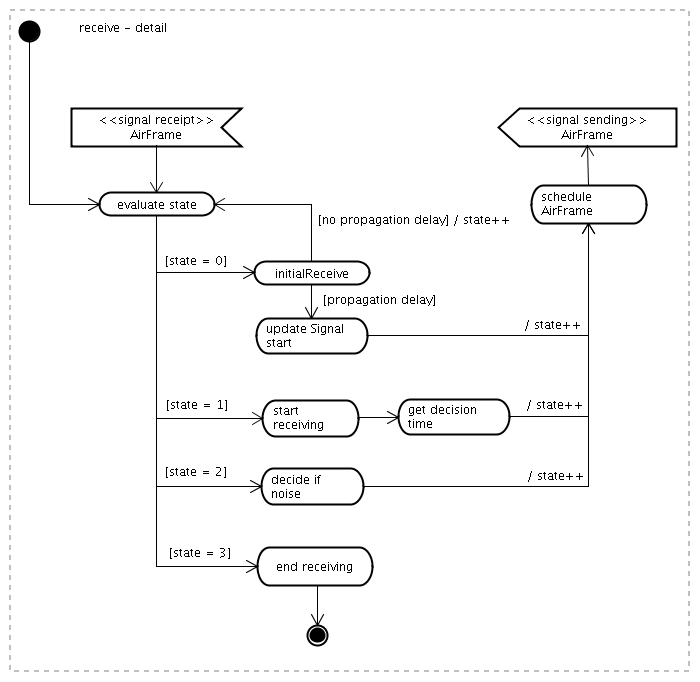
\includegraphics[width=340pt]{modelling/receive_detail.png}
 \caption{receive detail}
 \label{fig: receive detail}
\end{figure}

\begin{figure}[h]
 \centering
 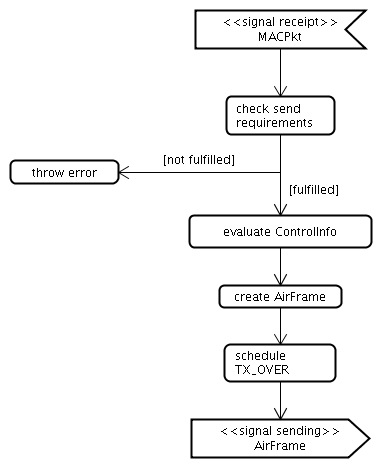
\includegraphics[width=300pt]{modelling/onMACPkt.png}
 \caption{sending process}
 \label{fig: sending process}
\end{figure}
